\documentclass[tikz]{standalone}
\begin{document}
    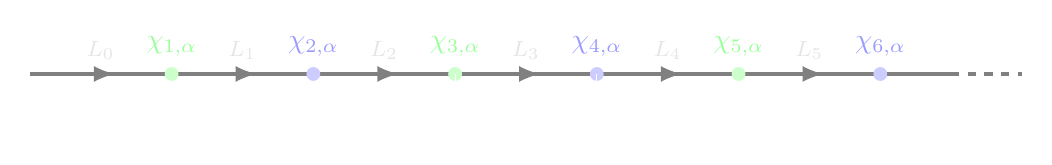
\begin{tikzpicture}[xscale=1.8]
        \draw[ultra thick,dashed,gray] (-1,0) -- (-.5,0);
        \draw[ultra thick,gray] (-.5,0) -- (5.5,0);
        \draw[ultra thick,dashed,gray] (5.5,0) -- (6,0);

        \foreach \x in {0,...,5} {
            \draw[ultra thick,-latex,gray] (\x - 1, 0) -- ({\x + .6 - 1},0);
            \node[gray!20!white] at ({\x - .5}, 0.3) {\footnotesize $L_\x$};
        }
        \foreach \x in {1,3,5} {
            \node[green!20!white,fill,circle,minimum size=5,inner sep=0,label=90:{\color{green!40!white} $\chi_{\x,\alpha}$}] at (\x-1, 0) {};
        }
        \foreach \x in {2,4,6} {
            \node[blue!20!white,fill,circle,minimum size=5,inner sep=0,label=90:{\color{blue!40!white} $\chi_{\x,\alpha}$}] at (\x-1, 0) {};
        }

        \draw[dashed,white] (2,0) -- (2,-.4) (3,0) -- (3,-.4);
        \draw[<->,thick,white] (2,-.4) -- node[below] {$a$} (3,-.4);
    \end{tikzpicture}
\end{document}